%%%%%%%%%%%%%%%%%%%%%%%%%%%%%%%%%%%%%%%%%%%%%%%%%%%%%%%%%%%%%%%%%%%%%%%%%%%

\documentclass{standalone}

\usepackage{amsmath}
\usepackage{mathptmx}
\usepackage{pgfplots}
\usetikzlibrary{external}
\tikzexternalize{rainbow-trout}
\pgfplotsset{compat=1.15}

%% IEEE uses Times Roman font, so we'll default to Times.
%% These three commands make up the entire times.sty package.
\renewcommand{\rmdefault}{ptm}
\renewcommand{\ttdefault}{pcr}
\normalfont\selectfont

\begin{document}

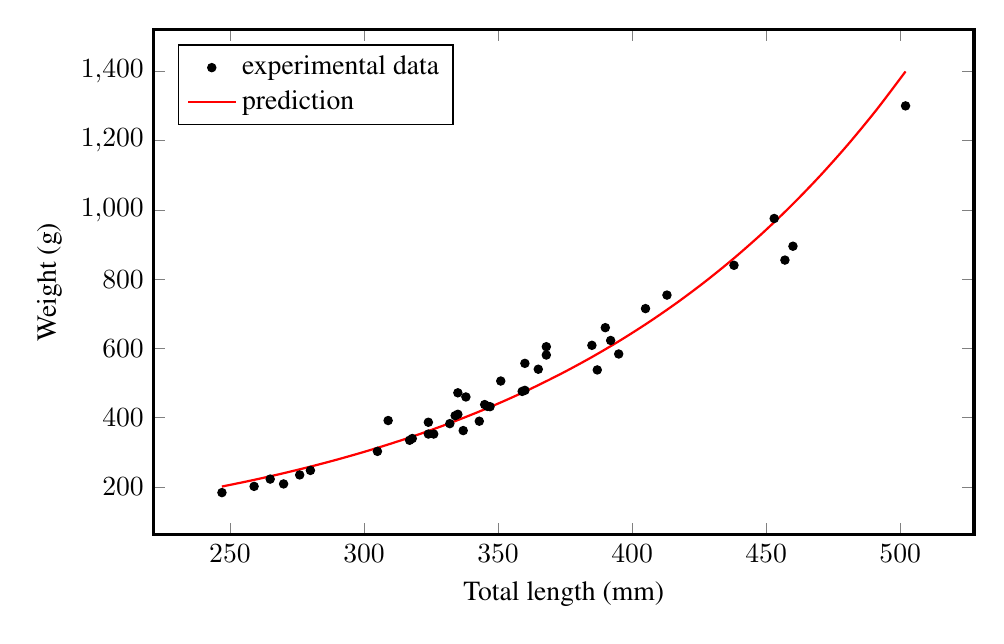
\begin{tikzpicture}
\tikzset{%%
  every mark/.append style={scale=1.0},%%
  scale=1.0%%
}
\pgfplotsset{%%
  every axis/.append style={font=\normalsize}%%
}
%%
\begin{axis}[%%
  axis line style=very thick,%%
  dotStyle/.style={mark size=1.5,black,mark color=black,mark=*,only marks},%%
  enlargelimits=true,%%
  height=8cm,%%
  legend cell align=left,%%
  legend pos=north west,%%
  plotStyle/.style={%%
    domain=247:502,%%
    mark=none,%%
    smooth,%%
    thick%%
  },%%
  width=12cm,%%
  %% x axis
  xlabel={\normalsize Total length~(mm)},%%
  %% y axis
  ylabel={\normalsize Weight~(g)}%%
]
%%
%%
\addplot[dotStyle] coordinates {
  (457, 855)
  (405, 715)
  (453, 975)
  (460, 895)
  (335, 472)
  (365, 540)
  (390, 660)
  (368, 581)
  (385, 609)
  (360, 557)
  (346, 433)
  (438, 840)
  (392, 623)
  (324, 387)
  (360, 479)
  (413, 754)
  (276, 235)
  (387, 538)
  (345, 438)
  (395, 584)
  (326, 353)
  (270, 209)
  (359, 476)
  (347, 432)
  (259, 202)
  (247, 184)
  (280, 248)
  (265, 223)
  (309, 392)
  (338, 460)
  (334, 406)
  (332, 383)
  (324, 353)
  (337, 363)
  (343, 390)
  (318, 340)
  (305, 303)
  (335, 410)
  (317, 335)
  (351, 506)
  (368, 605)
  (502, 1300)
};
\addlegendentry{experimental data}
%%
%%
\addplot+ [plotStyle,red]
{30.8338 * exp(0.0076*x)};
\addlegendentry{prediction}
\end{axis}
\end{tikzpicture}

\end{document}
